% =====================================================================
% Semana 2 · S2.4 — Equivalente de Thévenin del sensor
% Fundamentos de Sistemas Electrónicos Analógicos (Ingeniería Aeroespacial)
% Compilar: pdflatex semana_2_s24_thevenin_sensor.tex  (2 pasadas)
% =====================================================================
\documentclass[aspectratio=169]{beamer}

\usepackage[utf8]{inputenc}
\usepackage[T1]{fontenc}
\usepackage{lmodern}
\usepackage[spanish,es-tabla]{babel}
\usepackage{amsmath,amssymb}
\usepackage{siunitx}
\usepackage{booktabs}
\usepackage{microtype}
\usepackage{circuitikz}

\definecolor{navy}{RGB}{23,54,93}
\definecolor{navysoft}{RGB}{72,101,140}
\definecolor{gold}{RGB}{179,142,62}
\definecolor{ink}{RGB}{44,51,58}
\definecolor{soft}{RGB}{244,241,234}

\usetheme{default}
\setbeamertemplate{navigation symbols}{}
\setbeamertemplate{footline}[frame number]
\setbeamercolor{structure}{fg=navy}
\setbeamercolor{frametitle}{fg=white,bg=navy}
\setbeamercolor{title}{fg=navy}
\setbeamercolor{subtitle}{fg=navysoft}
\setbeamercolor{itemize item}{fg=gold}
\setbeamercolor{itemize subitem}{fg=gold}
\setbeamercolor{block title}{fg=white,bg=navy}
\setbeamercolor{block body}{bg=soft}
\setbeamercolor{example text}{fg=navy}
\setbeamertemplate{itemize item}{\scriptsize\raise1.25pt\hbox{\donotcoloroutermaths$\bullet$}}
\setbeamertemplate{itemize subitem}{\scriptsize\raise1.25pt\hbox{\donotcoloroutermaths$\circ$}}
\setbeamerfont{frametitle}{size=\large,series=\bfseries}

\title[S2.4 · Thévenin del sensor]{Equivalente de Thévenin del sensor}
\subtitle{S2.4 — Simulaciones y laboratorio de la Semana 2}
\institute{Licenciatura en Ingeniería Aeroespacial\\ UNAM · ENES Unidad Juriquilla}
\author{M. en C. José de Jesús Santana Ramírez}
\date{Semestre 2027-1}

\begin{document}

% ---------------------------------------------------------------------
\begin{frame}[plain]
  \titlepage
\end{frame}

% ---------------------------------------------------------------------
\begin{frame}{Objetivos de la sesión}
  \begin{itemize}
    \item Obtener el \textbf{equivalente de Thévenin} de una red resistiva de sensor: $V_{th}$ y $R_{th}$.
    \item Calcular $V_{th}$, $R_{th}$ e $I_n$ (Norton) desde la salida del divisor.
    \item Verificar que la red original y su equivalente \textbf{entregan la misma salida} a una carga.
    \item Usar el equivalente como \textbf{interfaz} con la siguiente etapa (amplificador o ADC).
  \end{itemize}
  \pause
  \begin{block}{Idea}
    El equivalente no es un truco algebraico: resume \emph{lo que ve} la siguiente etapa.
  \end{block}
\end{frame}

% ---------------------------------------------------------------------
\begin{frame}{Teoría 1 · Obtención de $V_{th}$ y $R_{th}$}
  Desde los terminales de salida del divisor:
  \[
    V_{th} = V_{in}\cdot\frac{R_2}{R_1+R_2}
    \qquad\qquad
    R_{th} = R_1\parallel R_2
    \qquad\qquad
    I_n = \frac{V_{th}}{R_{th}}
  \]
  \pause
  \begin{itemize}
    \item $V_{th}$: tensión en circuito \textbf{abierto} (sin carga).
    \item $R_{th}$: resistencia vista desde la salida con las \textbf{fuentes anuladas}
      (fuente de tensión $\rightarrow$ cortocircuito).
    \item $I_n$ (Norton): corriente de \textbf{cortocircuito} en la salida.
  \end{itemize}
\end{frame}

% ---------------------------------------------------------------------
\begin{frame}{Teoría 2 · Por qué sirve el equivalente}
  \begin{itemize}
    \item Permite calcular la salida con cualquier carga sin conservar toda la red:
      \[
        V_{out} = V_{th}\cdot\frac{R_L}{R_{th}+R_L}
      \]
    \item Permite calcular corriente de cortocircuito, disipación y \textbf{compatibilidad de impedancias}.
    \item Es la base de la \emph{ficha de interfaz}: se documenta $V_{th}$, $R_{th}$ y la carga admisible.
    \item Si $R_L \gg R_{th}$, la salida se mantiene cerca de $V_{th}$ (criterio de no carga, ver S2.1).
  \end{itemize}
\end{frame}

% ---------------------------------------------------------------------
\begin{frame}{Ejercicio · Enunciado}
  \begin{block}{Divisor de sensor frente a su equivalente}
    \centering
    $V_{in} = \SI{5}{\volt}$, $R_1 = R_2 = \SI{1}{\kilo\ohm}$; \quad equivalente: $V_{th} = \SI{2.5}{\volt}$, $R_{th} = \SI{500}{\ohm}$.
  \end{block}
  \begin{center}
    \resizebox{0.6\linewidth}{!}{%
    \begin{circuitikz}[american voltages, scale=0.85]
      \draw (0,3) to[V, l={$V_{in}=5\,\mathrm{V}$}, i=$I$] (0,0);
      \draw (0,3) -- (1.0,3) to[R, l={$R_1=1\,\mathrm{k}\Omega$}] (3.0,3);
      \draw (3.0,3) -- (5.4,3);
      \draw (3.7,3) to[R, l={$R_2$}] (3.7,0);
      \draw (5.0,3) to[R, l={$R_{L}$}] (5.0,0);
      \draw (0,0) -- (5.4,0);
      \node[circle, fill=gold, inner sep=0.9pt] at (3.0,3) {};
      \node[below, text=gold] at (3.0,2.7) {$V_{out}$};
    \node[ground] at (0,0) {};
    \end{circuitikz}}
  \end{center}
  \textbf{Verificar:} que ambas redes entregan la misma salida para $R_L = 1\,\text{k}$, $10\,\text{k}$, $100\,\text{k}$.
\end{frame}

% ---------------------------------------------------------------------
\begin{frame}{Desarrollo · Paso 1 — Calcular el equivalente}
  \[
    V_{th} = 5\cdot\frac{1000}{1000+1000} = \SI{2.5}{\volt}
    \qquad
    R_{th} = 1000\parallel 1000 = \SI{500}{\ohm}
    \qquad
    I_n = \frac{2.5}{500} = \SI{5}{\milli\ampere}
  \]
  \pause
  \begin{itemize}
    \item $I_n = \SI{5}{\milli\ampere}$ es la corriente de cortocircuito de la salida del divisor.
    \item Con estos dos parámetros queda definida la interfaz vista por la siguiente etapa.
  \end{itemize}
\end{frame}

% ---------------------------------------------------------------------
\begin{frame}{Desarrollo · Paso 2 — $R_L = \SI{1}{\kilo\ohm}$}
  \begin{align*}
    V_{out}^{orig} &= 5\cdot\frac{1000\parallel 1000}{1000 + (1000\parallel 1000)}
                     = 5\cdot\frac{500}{1500} = \SI{1.667}{\volt}\\[2pt]
    V_{out}^{eq} &= 2.5\cdot\frac{1000}{500+1000} = \SI{1.667}{\volt}
  \end{align*}
  \[
    \text{diferencia} = 0 \qquad\checkmark
  \]
\end{frame}

% ---------------------------------------------------------------------
\begin{frame}{Desarrollo · Paso 3 — $R_L = \SI{10}{\kilo\ohm}$}
  \begin{align*}
    V_{out}^{orig} &= 5\cdot\frac{1000\parallel 10000}{1000 + (1000\parallel 10000)}
                     = 5\cdot\frac{909.1}{1909.1} = \SI{2.381}{\volt}\\[2pt]
    V_{out}^{eq} &= 2.5\cdot\frac{10000}{500+10000} = \SI{2.381}{\volt}
  \end{align*}
  \[
    \text{diferencia} = 0 \qquad\checkmark
  \]
  \pause
  \begin{itemize}
    \item La carga ya no es despreciable: la salida cae de $2.5\,\text{V}$ a $2.381\,\text{V}$ (error de carga).
  \end{itemize}
\end{frame}

% ---------------------------------------------------------------------
\begin{frame}{Desarrollo · Paso 4 — $R_L = \SI{100}{\kilo\ohm}$}
  \begin{align*}
    V_{out}^{orig} &= 5\cdot\frac{1000\parallel 100000}{1000 + (1000\parallel 100000)}
                     = 5\cdot\frac{990.1}{1990.1} = \SI{2.4876}{\volt}\\[2pt]
    V_{out}^{eq} &= 2.5\cdot\frac{100000}{500+100000} = \SI{2.4876}{\volt}
  \end{align*}
  \[
    \text{diferencia} = 0 \qquad\checkmark
  \]
  \pause
  \begin{itemize}
    \item Con carga alta la salida se acerca a $V_{th} = 2.5\,\text{V}$ (poco error de carga).
  \end{itemize}
\end{frame}

% ---------------------------------------------------------------------
\begin{frame}{Desarrollo · Paso 5 — Verificación y lectura}
  \begin{table}
    \small
    \begin{tabular}{lccc}
      \toprule
      $R_L$ & $V_{out}^{orig}$ & $V_{out}^{eq}$ & Diferencia \\
      \midrule
      $\SI{1}{\kilo\ohm}$  & $\SI{1.667}{\volt}$ & $\SI{1.667}{\volt}$ & $0$ \\
      $\SI{10}{\kilo\ohm}$ & $\SI{2.381}{\volt}$ & $\SI{2.381}{\volt}$ & $0$ \\
      $\SI{100}{\kilo\ohm}$& $\SI{2.488}{\volt}$ & $\SI{2.488}{\volt}$ & $0$ \\
      \bottomrule
    \end{tabular}
  \end{table}
  \pause
  \begin{block}{Conclusión}
    El equivalente de Thévenin \textbf{reproduce exactamente} la salida de la red original
    para cualquier carga. Por eso la siguiente etapa analiza sólo ``una fuente de $V_{th}$
    con $R_{th}$ en serie'' y dimensiona su entrada con $R_{in} \gg R_{th}$.
  \end{block}
\end{frame}

% ---------------------------------------------------------------------
\begin{frame}[fragile]{Verificación en LTspice}
  Abrir \texttt{semana2\_04\_thevenin\_sensor.cir} (barrido de $R_L$: $1\,\text{k}$, $10\,\text{k}$, $100\,\text{k}$)
  y consultar el Error Log:

  \begin{verbatim}
.meas op V_ORIGINAL   FIND V(original)
.meas op V_EQUIVALENT FIND V(equivalent)
.meas op DIFFERENCE   PARAM V(original)-V(equivalent)
  \end{verbatim}

  \textbf{Criterio de éxito:} \texttt{DIFFERENCE} $\approx 0$ para las tres cargas.
\end{frame}

% ---------------------------------------------------------------------
  % ---------------------------------------------------------------------
  \begin{frame}{Resultado de la simulación}
    \begin{center}
      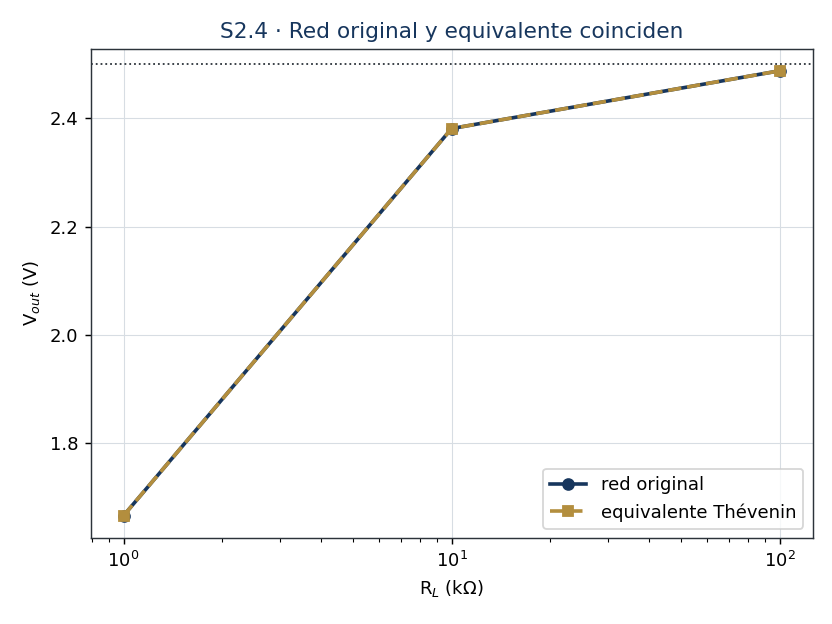
\includegraphics[width=0.78\textwidth]{figs/s24_thevenin.png}
    \end{center}
    \begin{itemize}
      \item La red original y el equivalente coinciden exactamente para toda carga.
    \end{itemize}
  \end{frame}

  % ---------------------------------------------------------------------
  \begin{frame}{Errores comunes}
  \begin{table}
    \small
    \begin{tabular}{p{0.34\textwidth}p{0.30\textwidth}p{0.30\textwidth}}
      \toprule
      Error & Consecuencia & Corrección \\
      \midrule
      Calcular $R_{th}$ sin anular la fuente & $R_{th}$ incorrecta & Fuente de tensión $\rightarrow$ cortocircuito \\
      Confundir $V_{th}$ con la salida cargada & La salida ya no es $V_{th}$ & $V_{th}$ es en circuito abierto \\
      Olvidar que la carga modifica la salida & Interfaz mal dimensionada & $V_{out} = V_{th}\,R_L/(R_{th}+R_L)$ \\
      No considerar $R_{out}$ de la rama & Error en el presupuesto & Usar $R_{th}$ en el modelo \\
      \bottomrule
    \end{tabular}
  \end{table}
\end{frame}

% ---------------------------------------------------------------------
\begin{frame}{Lectura aeroespacial}
  \begin{itemize}
    \item \textbf{Ficha de interfaz de sensor:} se documentan $V_{th}$, $R_{th}$, rango de $V_{diff}$,
      modo común, potencia y carga admisible. Es el contrato entre la etapa del sensor y la de amplificación.
    \item \textbf{Amplificación de instrumentación:} la $R_{in}$ del amplificador debe ser $\gg R_{th}$
      para no cargar el puente; el equivalente permite dimensionarla.
    \item \textbf{Compatibilidad de impedancias:} en la cadena sensor $\rightarrow$ acondicionador
      $\rightarrow$ ADC, cada etapa ``ve'' el equivalente de la anterior.
    \item \textbf{Corriente de cortocircuito:} $I_n$ ayuda a dimensionar protecciones (entrada del ADC)
      y a estimar la corriente máxima que puede entregar la interfaz.
  \end{itemize}
\end{frame}

% ---------------------------------------------------------------------
\begin{frame}{Preguntas de verificación}
  \begin{enumerate}
    \item ¿Qué es $V_{th}$: la salida con carga o en circuito abierto?
      \uncover<2->{\emph{(En circuito abierto.)}}
    \item ¿Cómo se anula una fuente de tensión para calcular $R_{th}$?
      \uncover<3->{\emph{(Cortocircuito; una fuente de corriente se abre.)}}
    \item ¿Por qué la red original y el equivalente dan la misma salida a cualquier carga?
      \uncover<4->{\emph{(Mismo $V_{th}$ y misma $R_{th}$ vistos por la carga.)}}
    \item Con $R_{th} = 500\,\Omega$ y $R_{in} = 10\,\text{k}\Omega$: ¿cuánto error de carga hay?
      \uncover<5->{\emph{($V_{out} = 2.5\cdot 10000/10500 = \SI{2.381}{\volt}$: error $\approx 4.8\,\text{\%}$.)}}
    \item ¿Por qué conviene $R_{in} \gg R_{th}$ en una interfaz de sensor?
  \end{enumerate}
\end{frame}


\end{document}
